\section{Examples with the packages \tkzname{alterqcm} and \tkzname{tkz-tab}}

\begin{alterqcm}[lq=110mm]

\AQmessage{Figure 1 shows the graph of a function $f$ defined on $[0, +\infty)$ and figure 2 the graph of an antiderivative of $f$ on $[0, +\infty)$.

\begin{center}
 \begin{tikzpicture}[xscale=2.25,yscale=1]
   \tkzFnInit[xmin=-2,xmax=3,ymin=-1,ymax=6]
   \tkzFnAxes[ticks=false]
   \tkzFnDraw[samples=100,domain=-1:2.2]{x+exp(x-1)}
   \tkzFnDefPointXY[draw](1,2){pt1}
   \tkzFnShowCoord[xlabel=$1$,ylabel=$2$](pt1)
   \tkzFnDefPointXY[draw](2,2+e){pt2}
   \tkzFnShowCoord[xlabel=$2$,ylabel=$\text{e}+2$](pt2)
   \tkzFnRep
 \end{tikzpicture}
\end{center}

\begin{center}
  \begin{tikzpicture}[xscale=2.25,yscale=1]
   \tkzFnInit[xmin=-2,xmax=3,ymin=-1,ymax=6]
   \tkzFnAxes[ticks=false]
   \tkzFnDraw[samples=100,domain=-1:2.2]{x*x/2+exp(x-1)}
   \tkzFnDefPointXY[draw](1,1.5){pt1}
   \tkzFnShowCoord[xlabel=$1$,ylabel=$3/2$](pt1)
   \tkzFnDefPointXY[draw](2,2+e){pt2}
   \tkzFnShowCoord[xlabel=$2$,ylabel=$\text{e}+2$](pt2)
   \tkzFnRep
\end{tikzpicture}
\end{center}}

\AQquestion{What is the area, in square units, of the region bounded by the graph of $f$, the $x$-axis and the lines $x = 1$ and $x = 2$?}
{{$\text{e} + \cfrac{3}{4}$},
{$\text{e} + \cfrac{1}{2}$},
{$1$}
}
\end{alterqcm}

\begin{alterqcm}[lq=90mm,pre=false,numbreak=1]
\AQmessage{The function $k$, defined and positive on $[0, +\infty)$, is given by its variation table.

\begin{center}
\begin{tikzpicture}
     \tkzTabInit[lgt=1,espcl=2]{$x$/0.5,$k(x)$/1.5}
     {$0$,$1$,$3$,$+\infty$}
     \tkzTabVar{-/            /,%
                +/            /,%
                -/            /,%
                +/ $+\infty$  /}%
\end{tikzpicture}
\end{center}%
}

\AQquestion{Which of the following tables is the variation table of the function $g$ defined on
$[0, +\infty)$ by \[g(x) = \cfrac{1}{k(x)}\ ? \]}
{{Table A},
{Table B},
{Table C}
}

\AQmessage{
\begin{center}
  Table A

\begin{tikzpicture}
     \tkzTabInit[lgt=1,espcl=2]{$x$/0.5,$g(x)$/1.5}
     {$0$,$1$,$3$,$+\infty$}
     \tkzTabVar{-/            /,%
                +/            /,%
                -/            /,%
                +/ $+\infty$  /}%
\end{tikzpicture}
\end{center}

\begin{center}
Table B

\begin{tikzpicture}
     \tkzTabInit[lgt=1,espcl=2]{$x$/0.5,$g(x)$/1.5}
     {$0$,$1$,$3$,$+\infty$}
     \tkzTabVar{+/            /,%
                -/            /,%
                +/            /,%
                -/ $-\infty$  /}%
\end{tikzpicture}
\end{center}

\begin{center}
Table C

\begin{tikzpicture}
     \tkzTabInit[lgt=1,espcl=2]{$x$/0.5,$g(x)$/1.5}
     {$0$,$1$,$3$,$+\infty$}
     \tkzTabVar{-/            /,%
                +/            /,%
                -/            /,%
                +/ $0$        /}%
\end{tikzpicture}
\end{center}
}

\AQquestion{Let $h$ be the function defined on $\mathbf{R}$ by $h(x) = \text{e}^x - x + 1$, and
$\mathcal{C}$ its graph in an orthonormal coordinate system $(O;\vec{\imath},\vec{\jmath})$.}
{{%
\begin{minipage}{5cm}
  The line $y = 1$ is an
  asymptote of $\mathcal{C}$%
\end{minipage}
},
{\begin{minipage}{5cm}
 The line $x = 0$ is an
 asymptote of $\mathcal{C}$
\end{minipage}},
{\begin{minipage}{5cm}
 The line $y = -x + 1$ is an
 asymptote of $\mathcal{C}$
\end{minipage}}
}
\AQquestion{In economics, the marginal cost is the cost of producing one more unit, and it is
taken to be the derivative of the total cost.\\
In a company, a study shows that the marginal cost $C_{m}(q)$, in thousands of dollars,
as a function of the number $q$ of items produced is:
\[C_{m}(q) = 3q^2 - 10q + \cfrac{2}{q} + 20.\]
}
{{ $C_{r}(q) = q^3 - 5q^2 + 2\ln q + 20q + 9984$},
{$C_{r}(q) = q^3 - 5q^2 + 2\ln q + 20q - 6$},
{$C_{r}(q) = 6q - 10 - \cfrac{2}{q^2}$}
}

\end{alterqcm}

Here is the code of the graphs of $f$ and of its antiderivative:

\subsubsection{First graph}
\begin{tkzexample}[code only]
\begin{tikzpicture}[xscale=2.25,yscale=1]
  \tkzFnInit[xmin=-2,xmax=3,ymin=-1,ymax=6]
  \tkzFnAxes[ticks=false]
  \tkzFnDraw[samples=100,domain=-1:2.2]{x+exp(x-1)}
  \tkzFnDefPointXY[draw](1,2){pt1}
  \tkzFnShowCoord[xlabel=$1$,ylabel=$2$](pt1)
  \tkzFnDefPointXY[draw](2,2+e){pt2}
  \tkzFnShowCoord[xlabel=$2$,ylabel=$\text{e}+2$](pt2)
  \tkzFnRep
\end{tikzpicture}
\end{tkzexample}

\subsubsection{Second graph}
\begin{tkzexample}[]
\begin{tikzpicture}[xscale=2.25,yscale=1]
  \tkzFnInit[xmin=-2,xmax=3,ymin=-1,ymax=6]
  \tkzFnAxes[ticks=false]
  \tkzFnDraw[samples=100,domain=-1:2.2]{x*x/2+exp(x-1)}
  \tkzFnDefPointXY[draw](1,1.5){pt1}
  \tkzFnShowCoord[xlabel=$1$,ylabel=$3/2$](pt1)
  \tkzFnDefPointXY[draw](2,2+e){pt2}
  \tkzFnShowCoord[xlabel=$2$,ylabel=$\text{e}+2$](pt2)
  \tkzFnRep
\end{tikzpicture}
\end{tkzexample}

The answer to the first question can be checked with Lua: $\int_1^2 f(x)\,\text{d}x\approx\tkzFnPrint[4]{integral("x+exp(x-1)",1,2)}$ and $\text{e}+\frac12\approx\tkzFnPrint[4]{e+1/2}$.

Code of a variation table:

\begin{tkzltxexample}[]
\begin{tikzpicture}
     \tkzTabInit[lgt=1,espcl=2]{$x$/0.5,$k(x)$/1.5}
     {$0$,$1$,$3$,$+\infty$}
     \tkzTabVar{-/            /,%
                +/            /,%
                -/            /,%
                +/ $+\infty$  /}%
\end{tikzpicture}
\end{tkzltxexample}

\endinput
